\documentclass{article}

\usepackage{tikz}
\usepackage{amsmath}
\usetikzlibrary{math, patterns}

\begin{document}
    \begin{center}
        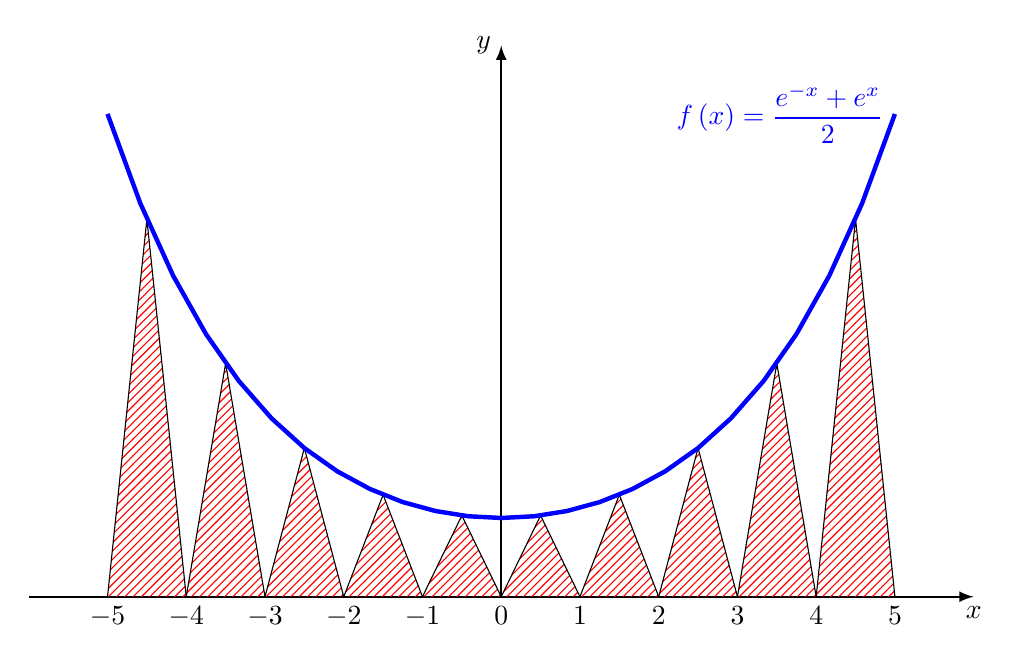
\begin{tikzpicture}
            \draw[->,>=latex,thick] (-6,0) -- (6,0) node[below]{\(x\)};
            \draw[->,>=latex,thick] (0,0) -- (0,7) node[left]{\(y\)};
            
            \tikzmath{
                function calcFValue(\x){
                    return 0.5*(e^(-0.5*\x) + e^(0.5*\x));
                };
            }

            \foreach \x in {-4,...,5}{
                \draw[pattern color=red, pattern=north east lines] 
                    (\x-1, 0) -- (\x-0.5, {calcFValue(\x-0.5)}) -- (\x, 0) 
                    node[below]{\(\x\)}; 
            }

            \draw[ultra thick, blue, domain=-5:5] 
                plot (\x, {0.5*(e^(-0.5*\x) + e^(0.5*\x))})
                node[left]{\(f\left(x\right)=\dfrac{e^{-x}+e^x}{2}\)};
            \node at (-5,0)[below]{\(-5\)};
        \end{tikzpicture}
        
    \end{center}
\end{document}